\label{methodology}
As seen, the literature on this topic is quite vast and explore a lot of different considerations regarding the operation and dimensioning of a REC. In this work, the objective is to focus on visualizing the fairness problematics in energy communities. For doing so, the choice has been to make a model of a REC where we can easily make two optimizations, one fully centralized with exchanges and one fully decentralized without exchanges. This way we should be able to compute the maximum gain that can be achieved by the community. The goal of this project is also to make the model easily customizable in order to be reused in future projects. Then we will implement different gain allocation functions that have different properties in terms of fairness. Finally, we will develop different visualization tools in order to understand the effect of the different gain allocation functions on the fairness within the community.

The figure \ref{fig:methodology} gives an overview of the community model. A community is made of several prosumers, that are themselves made out of several devices. This way we can first define a model of each type of device and flexibility services in a house. The models of devices consist of a set of variables and constraints. This way we easily build the model of a member of the community by simply aggregating the models of its devices. We still need to add to this model, as a variable, the power exchange with the community and the grid as well as the power balance constraint associated to it. By adding an objective function to this model, we can directly optimize the system in a fully decentralized way. To make the model of the community, in the same way, we just aggregate the models of the different members and we add the constraints related to the power exchange between the members. By adding an objective function to this model, we can optimize the system in a fully centralized way.

With this optimization built, we can compute the gain of the community. We then need to allocate these gains within the community. In this work, 3 allocation functions were chosen in order to represent the fairness problematics. The first one is the Shapley value, it focuses on the "meritocratic" fairness as seen in the state of the art. Then we choose the "egalitarian" allocation function, that gives the same gain to all the members of the community. Finally, the proportional allocation function that gives to each member a gain proportional to there contribution in reducing the global cost of the community. These three functions have very different properties in terms of fairness and are thus ideal to visualize the effect of the chosen function on a fair repartition of the gains.

The representation of the gains we thought of were mostly inspired by the radar charts shown in \cite{these_sorel}, but we wanted to add more information to them and to make them more interpretable. Another representation we thought of is a Pareto front of our the model regarding the sociological profile of the members of the community in order to visualize the influence of this sociological profile. The model has been built keeping these representations in mind, notably in order to plot a Pareto front.



\begin{figure}[h]
    \centering
    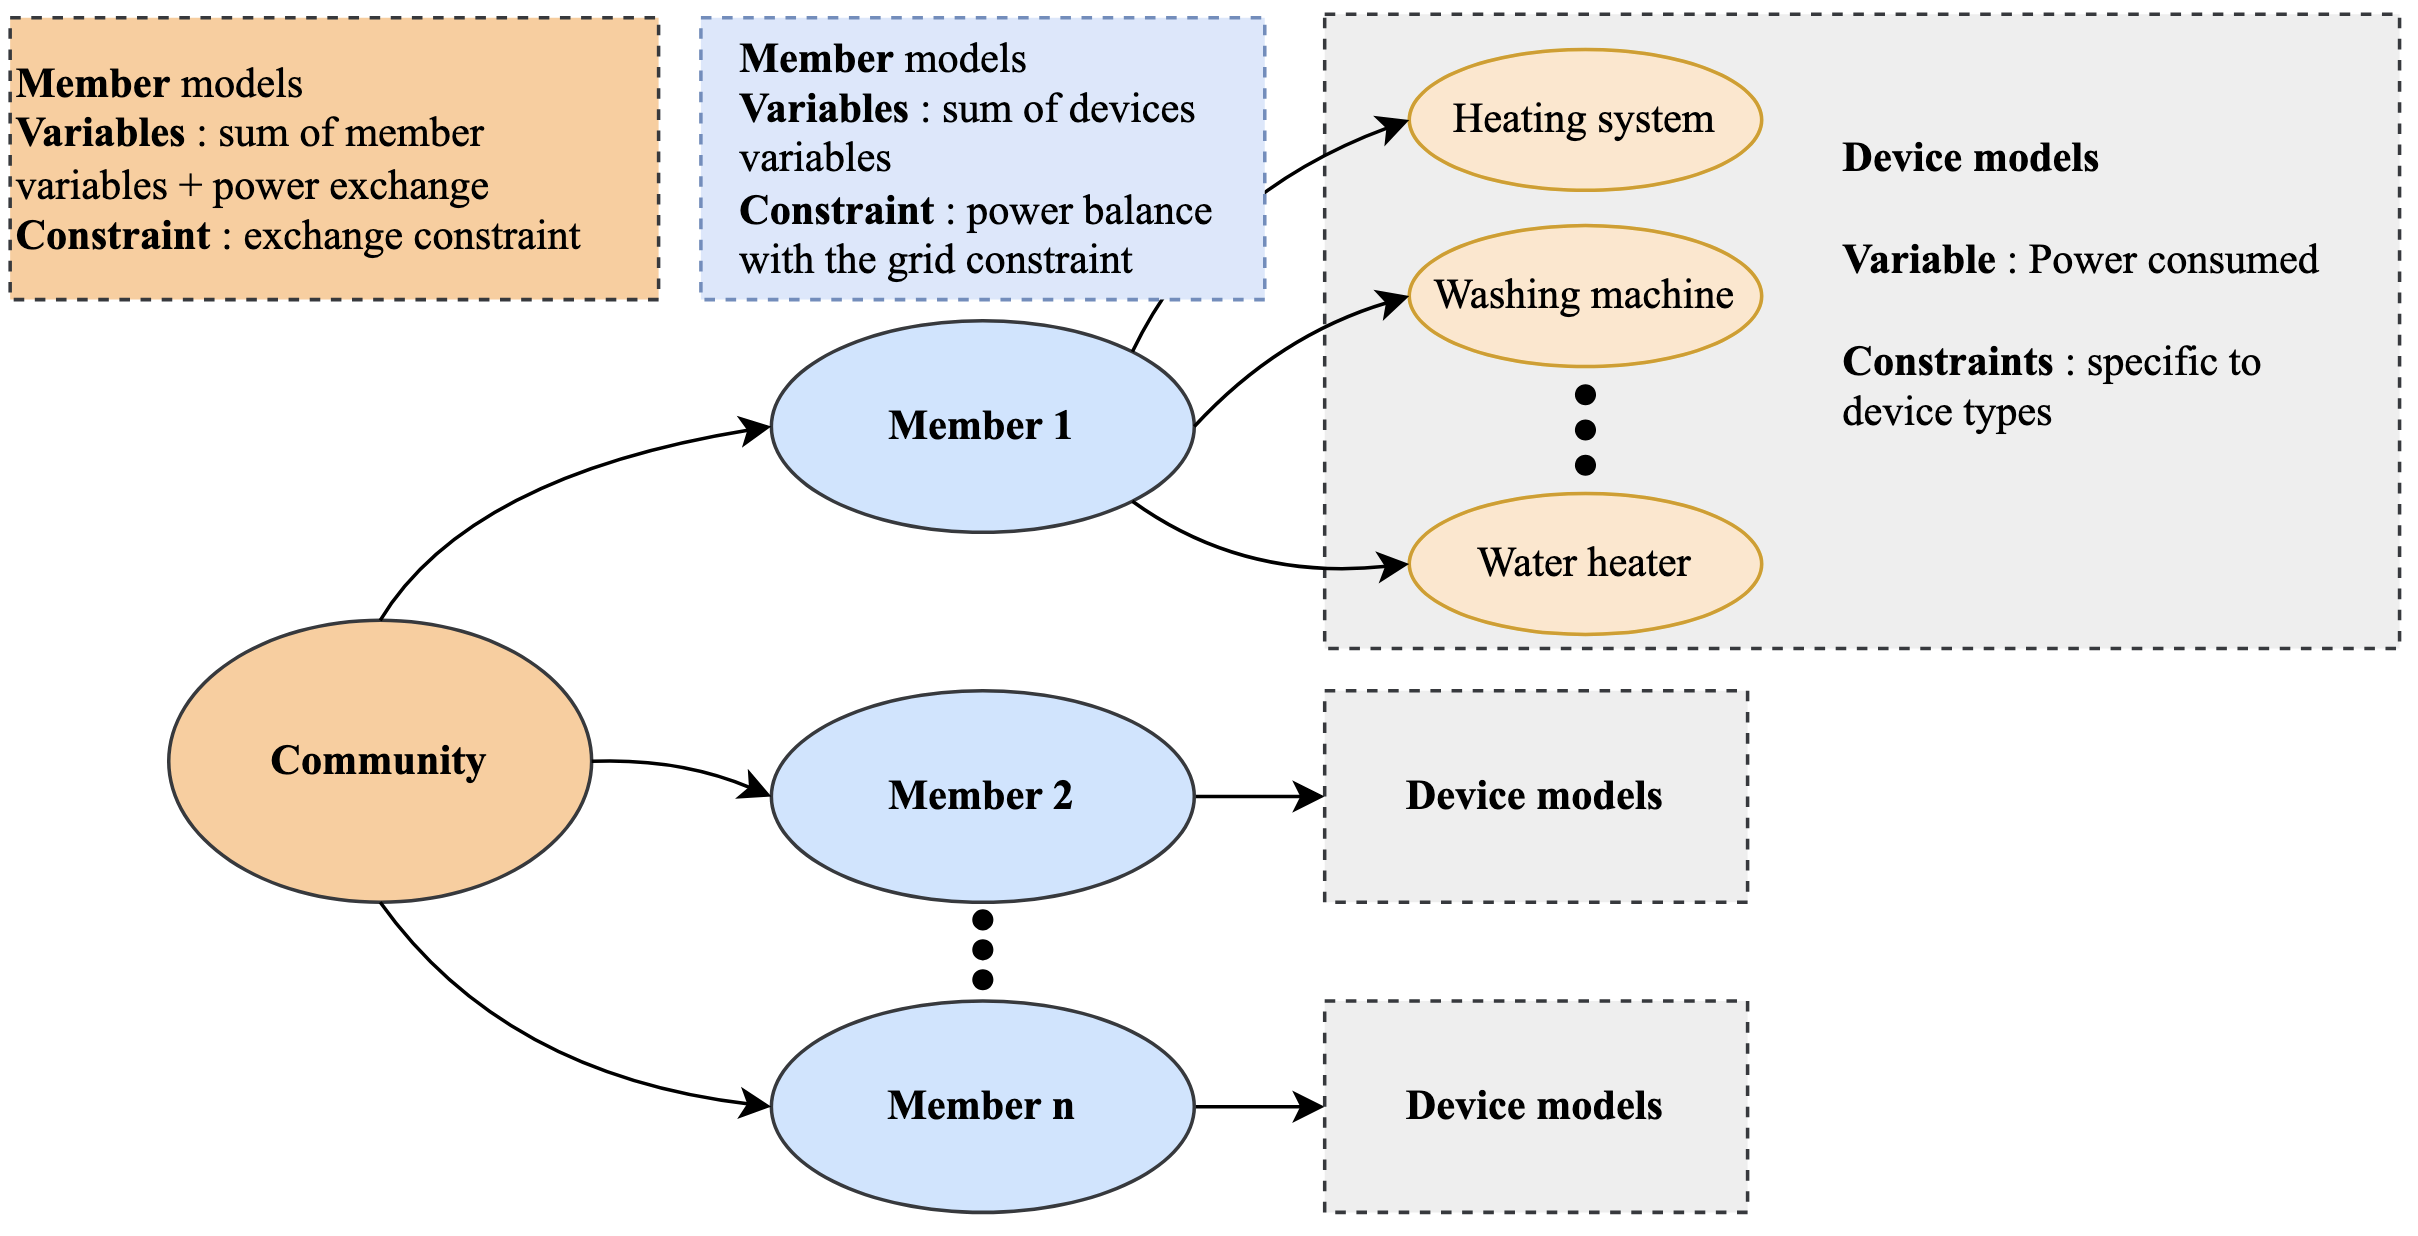
\includegraphics[width=\textwidth]{methodo.png}
    \caption{Model overview}
    \label{fig:methodology}
\end{figure}